%beamer

% Comment/uncomment this line to toggle handout mode
\newcommand{\handout}{}

%% Beamer-Klasse im korrekten Modus
\ifdefined \handout
\documentclass[handout]{beamer} % Handout mode
\else
\documentclass{beamer}
\fi

%% UTF-8-Encoding
\usepackage[utf8]{inputenc}

\input{../framework/gbi-macros}
\usepackage[blue]{../framework/thwregex}
\usepackage{environ}
\usepackage{bm}
\usepackage{calc}
\usepackage{varwidth}
\usepackage{wasysym}
\usepackage{mathtools}


% Das ist der KIT-Stil
%\usepackage{../TutTexbib/beamerthemekit}
\usepackage[deutsch,titlepage0]{../framework/KIT/beamerthemeKITmod}
\TitleImage[width=\titleimagewd]{../figures/titlepage.jpg}
%\usetheme[deutsch,titlepage0]{KIT}

% Include PDFs
\usepackage{pdfpages}

% Libertine font (Original GBI font)
\usepackage{libertine}
%\renewcommand*\familydefault{\sfdefault}  %% Only if the base font of the document is to be sans serif

% Nicer math symbols
\usepackage{eulervm}
%\usepackage{mathpazo}
\renewcommand\ttdefault{cmtt} % Computer Modern typewriter font, see lecture slides.

\usepackage{csquotes}

%%%%%%

%% Schönere Schriften
\usepackage[TS1,T1]{fontenc}

%% Bibliothek für Graphiken
\usepackage{graphicx}

%% der wird sowieso in jeder Datei gesetzt
\graphicspath{{../figures/}}

%% Anzeigetiefe für Inhaltsverzeichnis: 1 Stufe
\setcounter{tocdepth}{1}

%% Hyperlinks
\usepackage{hyperref}
% I don't know why, but this works and only includes sections and NOT subsections in the pdf-bookmarks.
\hypersetup{bookmarksdepth=subsection} 

%\usepackage{lmodern}
\usepackage{colortbl}
\usepackage[absolute,overlay]{textpos}
\usepackage{listings}
\usepackage{forloop}
%\usepackage{algorithmic} % PseudoCode package 

\usepackage{tikz}
\usetikzlibrary{matrix}
\usetikzlibrary{arrows.meta}
\usetikzlibrary{automata}
\usetikzlibrary{tikzmark}
\usetikzlibrary{positioning}

% Why has no-one come up with this yet? I mean, seriously. -.-
\tikzstyle{loop below right} = [loop, out=-60,in=-30, looseness=7]
\tikzstyle{loop below left} = [loop, out=-150,in=-120, looseness=7]
\tikzstyle{loop above right} = [loop, out=60,in=30, looseness=7]
\tikzstyle{loop above left} = [loop, out=150,in=120, looseness=7]
\tikzstyle{loop right below} = [loop below right]
\tikzstyle{loop left below} = [loop below left]
\tikzstyle{loop right above} = [loop above right]
\tikzstyle{loop left above} = [loop above left]

% Needed for gbi-macros
\usepackage{xspace}

%%%%%%

%% Verbatim
\usepackage{moreverb}

%%%%%%%%%%%%%%%%%%%%%%%%%%%%%%%%%%%% Copy end

%% Tabellen
\usepackage{array}
\usepackage{multicol}
\usepackage{hhline}

%% Bibliotheken für viele mathematische Symbole
\usepackage{amsmath, amsfonts, amssymb}

%% Deutsche Silbentrennung und Beschriftungen
\usepackage[ngerman]{babel}

\usepackage{kbordermatrix}

% kbordermatrix settings
\renewcommand{\kbldelim}{(} % Left delimiter
\renewcommand{\kbrdelim}{)} % Right delimiter

\input{../config.tex}



% define custom \handout command flag if handout mode is toggled  #DirtyAsHellButWell...
\only<beamer:0>{\def\handout{}} %beamer:0 == handout mode

\newcommand{\R}{\mathbb{R}}
\newcommand{\N}{\mathbb{N}}
\newcommand{\Z}{\mathbb{Z}}
\newcommand{\Q}{\mathbb{Q}}
\newcommand{\BB}{\mathbb{B}}
\newcommand{\C}{\mathbb{C}}
\newcommand{\K}{\mathbb{K}}
\newcommand{\G}{\mathbb{G}}
\newcommand{\nullel}{\mathcal{O}}
\newcommand{\einsel}{\mathds{1}}
\newcommand{\Pot}{\mathcal{P}}
\renewcommand{\O}{\text{O}}

\def\word#1{\hbox{\textcolor{blue}{\texttt{#1}}}}
\let\literal\word
\def\mword#1{\hbox{\textcolor{blue}{$\mathtt{#1}$}}}  % math word
\def\sp{\scalebox{1}[.5]{\textvisiblespace}}
\def\wordsp{\word{\sp}}

%\newcommand{\literal}[1]{\textcolor{blue}{\texttt{#1}}}
\newcommand{\realTilde}{\textasciitilde \ }
\newcommand{\setsize}[1]{\ensuremath{\left\lvert #1 \right\rvert}}
\newcommand{\size}[1]{\setsize{#1}}  % Shame on you, TeXStudio...
\newcommand{\set}[1]{\left\{#1\right\}}
\newcommand{\tuple}[1]{\left(#1\right)}
\newcommand{\normalvar}[1]{\text{$#1$}}

% Modified by DJ
\let\oldemptyset\emptyset
\let\emptyset\varnothing % proper emptyset

\newcommand{\boder}{\ensuremath{\mathbin{\textcolor{blue}{\vee}}}\xspace}
\newcommand{\bund}{\ensuremath{\mathbin{\textcolor{blue}{\wedge}}}\xspace}
\newcommand{\bimp}{\ensuremath{\mathrel{\textcolor{blue}{\to}}}\xspace}
\newcommand{\bgdw}{\ensuremath{\mathrel{\textcolor{blue}{\leftrightarrow}}}\xspace}
\newcommand{\bnot}{\ensuremath{\textcolor{blue}{\neg}}\xspace}
\newcommand{\bone}{\ensuremath{\textcolor{blue}{1}}\text{}}
\newcommand{\bzero}{\ensuremath{\textcolor{blue}{0}}\text{}}
\newcommand{\bleftBr}{\ensuremath{\textcolor{blue}{\texttt{(}}}\text{}}
\newcommand{\brightBr}{\ensuremath{\textcolor{blue}{\texttt{)}}}\text{}}

% Fix of \b... commands:

\renewcommand{\boder}{\alor}
\renewcommand{\bund}{\aland}
\renewcommand{\bimp}{\alimpl}
\renewcommand{\bgdw}{\aleqv}
\renewcommand{\bnot}{\alnot}
\renewcommand{\bleftBr}{\alka}
\renewcommand{\brightBr}{\alkz}
\newcommand{\alA}{\word A}
\newcommand{\alB}{\word B}
\newcommand{\alC}{\word C}

\newcommand{\plB}{\plfoo{B}}
\newcommand{\plE}{\plfoo{E}}

\newcommand{\summe}[2]{\sum\limits_{#1}^{#2}}
\newcommand{\limes}[1]{\lim\limits_{#1}}

%\newcommand{\numpp}{\advance \value{weeknum} by -2 \theweeknum \advance \value{weeknum} by 2}
%\newcommand{\nump}{\advance \value{weeknum} by -1 \theweeknum \advance \value{weeknum} by 1}

\newcommand{\mycomment}[1]{}
\newcommand{\Comment}[1]{}

%% DISCLAIMER START 
% It is INSANELY IMPORTANT NOT TO DO THIS OUTSIDE BEAMER CLASS! IN ARTCILE DOCUMENTS, THIS IS VERY LIKELY TO BUG AROUND!
\makeatletter%
\@ifclassloaded{beamer}%
{
	% TODO 
	% no time... later.   (= never -.-)
	% redefine section to ignore multiple \section calls with the same title
}%
{
	\errmessage{ERROR: section command redefinition outside of beamer class document! Please contact the author of this code or read the F-ing disclaimer.}
}%
\makeatother%
%% DISCLAIMER END

\newcounter{abc}
\newenvironment{alist}{
  \begin{list}{(\alph{abc})}{
      \usecounter{abc}\setlength{\leftmargin}{8mm}\setlength{\labelsep}{2mm}
    }
}{\end{list}}


\newcommand{\stdarraystretch}{1.20}
\renewcommand{\arraystretch}{\stdarraystretch}  % for proper row spacing in tables

\newcommand{\morescalingdelimiters}{   % for proper \left( \right) typography
	\delimitershortfall=-1pt  
	\delimiterfactor=1
}

\newcommand{\centered}[1]{\vspace{-\baselineskip}\begin{center}#1\end{center}\vspace{-\baselineskip}}

% for \implitem and \item[bla] stuff to look right:
\setbeamercolor*{itemize item}{fg=black}
\setbeamercolor*{itemize subitem}{fg=black}
\setbeamercolor*{itemize subsubitem}{fg=black}

\setbeamercolor*{description item}{fg=black}
\setbeamercolor*{description subitem}{fg=black}
\setbeamercolor*{description subsubitem}{fg=black}

\renewcommand{\qedsymbol}{\textcolor{black}{\openbox}}

\renewcommand{\mod}{\mathop{\textbf{mod}}}
\renewcommand{\div}{\mathop{\textbf{div}}}

\newcommand{\ceil}[1]{\left\lceil#1\right\rceil}
\newcommand{\floor}[1]{\left\lfloor#1\right\rfloor}
\newcommand{\abs}[1]{\left\lvert #1 \right\rvert}
\newcommand{\Matrix}[1]{\begin{pmatrix} #1 \end{pmatrix}}
\newcommand{\braced}[1]{\left\lbrace #1 \right\rbrace}

% "something" placeholder. Useful for repairing spacing of operator sections, like `\sth = 42`.
\def\sth{\vphantom{.}}

\def\fract#1/#2 {\frac{#1}{#2}} % ! Trailing space is crucial!
\def\dfract#1/#2 {\dfrac{#1}{#2}} % ! Trailing space is crucial!

\newcommand{\Mid}{\;\middle|\;}

\let\after\circ



\def\·{\cdot}
\def\*{\cdot}
\def\?>{\ensuremath{\rightsquigarrow}}  % Fuck you, Latex
\def\~~>{\ensuremath{\rightsquigarrow}}  

\newcommand{\tight}[1]{{\renewcommand{\arraystretch}{0.76} #1}}
\newcommand{\stackedtight}[1]{\renewcommand{\arraystretch}{0.76} \begin{matrix} #1 \end{matrix} }
\newcommand{\stacked}[1]{\begin{matrix} #1 \end{matrix} }
\newcommand{\casesl}[1]{\delimitershortfall=0pt  \left\lbrace\hspace{-.3\baselineskip}\begin{array}{ll} #1 \end{array}\right.}
\newcommand{\casesr}[1]{\delimitershortfall=0pt  \left.\begin{array}{ll} #1 \end{array}\hspace{-.3\baselineskip}\right\rbrace}
\newcommand{\caseslr}[1]{\delimitershortfall=0pt  \left\lbrace\hspace{-.3\baselineskip}\begin{array}{ll} #1 \end{array}\hspace{-.3\baselineskip}\right\rbrace}

\def\q#1uad{\ifnum#1=0\relax\else\quad\q{\the\numexpr#1-1\relax}uad\fi}
% e.g. \q1uad = \quad, \q2uad = \qquad etc.

\newcommand{\qqquad}{\q3uad}
\newcommand{\minusquad}{\hspace{-1em}}

%% Placeholder utils
% \§{#1}   Saves #1 as placeholder and prints it
% \.       Prints an \hphantom with the size of the recalled placeholder.
\def\indentstring{}
\def\§#1{\def\indentstring{#1}#1}
\def\.{{$\hphantom{\text{\indentstring}}$}}
%% Placeholder utils end

\newcommand{\impl}{\ifmmode\ensuremath{\mskip\thinmuskip\Rightarrow\mskip\thinmuskip}\else$\Rightarrow$\fi\xspace}
\newcommand{\Impl}{\ifmmode\implies\else$\Longrightarrow$\fi\xspace}

\newcommand{\derives}{\Rightarrow}

\newcommand{\gdw}{\ifmmode\mskip\thickmuskip\Leftrightarrow\mskip\thickmuskip\else$\Leftrightarrow$\fi\xspace}
\newcommand{\Gdw}{\ifmmode\iff\else$\Longleftrightarrow$\fi\xspace}

% Legacy code from the algo tutorial slides. Perhaps useful. Try with care.
\mycomment{
	\newcommand{\impl}{\ifmmode\ensuremath{\mskip\thinmuskip\Rightarrow\mskip\thinmuskip}\else$\Rightarrow$\xspace\fi}  
	\newcommand{\Impl}{\ifmmode\implies\else$\Longrightarrow$\xspace\fi}
	
	\newcommand{\gdw}{\ifmmode\mskip\thickmuskip\Leftrightarrow\mskip\thickmuskip\else$\Leftrightarrow$\xspace\fi}
	\newcommand{\Gdw}{\ifmmode\iff\else$\Longleftrightarrow$\xspace\fi}
}
	
\newcommand{\gdwdef}{\ifmmode\mskip\thickmuskip:\Leftrightarrow\mskip\thickmuskip\else:$\Leftrightarrow$\xspace\fi}
\newcommand{\Gdwdef}{\ifmmode\mskip\thickmuskip:\Longleftrightarrow\mskip\thickmuskip\else:$\Longleftrightarrow$\xspace\fi}

\newcommand{\symbitemnegoffset}{\hspace{-.5\baselineskip}}
\newcommand{\implitem}{\item[\impl\symbitemnegoffset]}
\newcommand{\Implitem}{\item[\Impl\symbitemnegoffset]}


\newcommand{\forcenewline}{\mbox{}\\}

\newcommand{\bfalert}[1]{\textbf{\alert{#1}}}
\let\elem\in   % I'm a Haskell freak. Don't judge me. :P


\def\|#1|{\text{\normalfont #1}}  % | steht für senkrecht (anstatt kursiv wie sonst im math mode)


% proper math typography
\newcommand{\functionto}{\longrightarrow}
\renewcommand{\geq}{\geqslant}
\renewcommand{\leq}{\leqslant}
\let\oldsubset\subset
\renewcommand{\subset}{\subseteq} % for all idiots out there using subset

\newenvironment{threealign}{%
	\[
	\begin{array}{r@{\ }c@{\ }l}
}{%
	\end{array}	
	\]
}

\newcommand{\concludes}{ \\ \hline  }
\newcommand{\deduction}[1]{
	\begin{varwidth}{.8\linewidth}
		\begin{tabular}{>{$}c<{$}}
			#1
		\end{tabular}
	\end{varwidth}	
}

\definecolor{hoareorange}{rgb}{1,.85,.6}
\newcommand{\hoareassert}[1]{\setlength{\fboxsep}{1pt}\setlength{\fboxrule}{-1.4pt}\fcolorbox{white}{hoareorange}{\ensuremath{\{\;#1\;\}}}\setlength\fboxrule{\defaultfboxrule}\setlength{\fboxsep}{3pt}}

\newcommand{\mailto}[1]{\href{mailto:#1}{{\textcolor{blue}{\underline{#1}}}}}
\newcommand{\urlnamed}[2]{\href{#2}{\textcolor{blue}{\underline{#1}}}}
\renewcommand{\url}[1]{\urlnamed{#1}{#1}}

\newcommand{\hanging}{\hangindent=0.7cm}
\newcommand{\indented}{\hanging}


% \hstretchto prints #2 left-aligned into a box of the width of #1
\def\hstretchto#1#2{%
	\mbox{}\vphantom{#2}\rlap{#2}\hphantom{#1}%
}

\def\vstretchto#1#2{%
	\mbox{}\hphantom{#2}\smash{#2}\vphantom{#1}%
}

% \hstretchtocentered prints #2 centered into a box of the width of #1
\def\hstretchtocentered#1#2{%
	\mbox{}\vphantom{#2}\scalebox{0.5}{\hphantom{#1}}\clap{#2}\scalebox{0.5}{\hphantom{#1}}%
}

% vertical centering
\newcommand{\vertcenter}[1]{%
	\ensuremath{\vcenter{\hbox{#1}}}%
}


%requires \thisyear to be defined (s. config.tex)!
\edef\nextyear{\the\numexpr\thisyear+1\relax}


% --- \frameheight constant ---
\newlength\fullframeheight
\newlength\framewithtitleheight
\setlength\fullframeheight{.92\textheight}
\setlength\framewithtitleheight{.86\textheight}

\newlength\frameheight
\setlength\frameheight{\fullframeheight}

\let\frametitleentry\relax
\let\oldframetitle\frametitle
\def\newframetitle#1{\global\def\frametitleentry{#1}\if\relax\frametitleentry\relax\else\setlength\frameheight{\framewithtitleheight}\fi\oldframetitle{#1}}
\let\frametitle\newframetitle

\def\newframetitleoff{\let\frametitle\oldframetitle}
\def\newframetitleon{\let\frametitle\newframetitle}
% --- \frameheight constant end ---

\newcommand{\fakeframetitle}[1]{%
	\vspace{-2.05\baselineskip}%
	{\Large \textbf{#1}} \\%
	\smallskip
}



\newenvironment{headframe}{\Huge THIS IS AN ERROR. PLEASE CONTACT THE ADMIN OF THIS TEX CODE. (headframe env def failed)}{}
\RenewEnviron{headframe}[1][]{
	\begin{frame}\frametitle{\ }
		\centering
		\Huge\textbf{\textsc{\BODY} \\
		}
		\Large {#1}
		\frametitle{\ }
	\end{frame}
}


\makeatletter
% Provides color if undefined.
\newcommand{\colorprovide}[2]{%
	\@ifundefinedcolor{#1}{\colorlet{#1}{#2}}{}}
\makeatother


\colorprovide{lightred}{red!30}
\colorprovide{lightgreen}{green!40}
\colorprovide{lightyellow}{yellow!50}
\colorprovide{lightblue}{blue!10}
\colorprovide{beamerlightred}{lightred}
\colorprovide{beamerlightgreen}{lightgreen}
\colorprovide{beamerlightyellow}{lightyellow}
\colorprovide{beamerlightblue}{lightblue}
\colorprovide{fullred}{red!60}
\colorprovide{fullgreen}{green}
\definecolor{darkred}{RGB}{115,48,38}
\definecolor{darkgreen}{RGB}{48,115,38}
\definecolor{darkyellow}{RGB}{100,100,0}

\only<handout:0>{\colorlet{adaptinglightred}{beamerlightred}}
\only<handout:0>{\colorlet{adaptinglightgreen}{beamerlightgreen}}
\only<handout:0>{\colorlet{adaptinglightyellow}{beamerlightyellow}}
\only<handout:0>{\colorlet{adaptinglightblue}{beamerlightblue}}
\only<beamer:0>{\colorlet{adaptinglightred}{lightred}}
\only<beamer:0>{\colorlet{adaptinglightgreen}{lightgreen}}
\only<beamer:0>{\colorlet{adaptinglightyellow}{lightyellow}}
\only<beamer:0>{\colorlet{adaptinglightblue}{lightblue}}
\only<handout:0>{\colorlet{adaptingred}{lightred}}
\only<beamer:0>{\colorlet{adaptingred}{fullred}}
\only<handout:0>{\colorlet{adaptinggreen}{lightgreen}}
\only<beamer:0>{\colorlet{adaptinggreen}{fullgreen}}



\newcommand{\TrueQuestion}[1]{
	\TrueQuestionE{#1}{}
}

\newcommand{\YesQuestion}[1]{
	\YesQuestionE{#1}{}
}

\newcommand{\FalseQuestion}[1]{
	\FalseQuestionE{#1}{}
}

\newcommand{\NoQuestion}[1]{
	\NoQuestionE{#1}{}
}

\newcommand{\DependsQuestion}[1]{
	\DependsQuestionE{#1}{}
}

\newcommand{\QuestionVspace}{\vspace{4pt}}
\newcommand{\QuestionParbox}[1]{\begin{varwidth}{.85\linewidth}#1\end{varwidth}}
\newcommand{\ExplanationParbox}[1]{\begin{varwidth}{.97\linewidth}#1\end{varwidth}}
\colorlet{questionlightgray}{gray!23}
\let\defaultfboxrule\fboxrule

% #1: bg color
% #2: fg color short answer
% #3: short answer text
% #4: question
% #5: explanation
\newcommand{\GenericQuestion}[5]{
	\setlength\fboxrule{2pt}
	\only<+|handout:0>{\hspace{-2pt}\fcolorbox{white}{questionlightgray}{\QuestionParbox{#4} \quad\textbf{?}}}
	\visible<+->{\hspace{-2pt}\fcolorbox{white}{#1}{\QuestionParbox{#4} \quad\textbf{\textcolor{#2}{#3}}} \if\relax#5\relax\else\ExplanationParbox{#5}\fi} \\
	\setlength\fboxrule{\defaultfboxrule}
}

% #1: Q text
% #2: Explanation
\newcommand{\TrueQuestionE}[2]{
	\GenericQuestion{adaptinglightgreen}{darkgreen}{Wahr.}{#1}{#2}
}

% #1: Q text
% #2: Explanation
\newcommand{\YesQuestionE}[2]{
	\GenericQuestion{adaptinglightgreen}{darkgreen}{Ja.}{#1}{#2}
}

% #1: Q text
% #2: Explanation
\newcommand{\FalseQuestionE}[2]{
	\GenericQuestion{adaptinglightred}{darkred}{Falsch.}{#1}{#2}
}

% #1: Q text
% #2: Explanation
\newcommand{\NoQuestionE}[2]{
	\GenericQuestion{adaptinglightred}{darkred}{Nein.}{#1}{#2}
}

% #1: Q text
% #2: Explanation
\newcommand{\DependsQuestionE}[2]{
	\GenericQuestion{adaptinglightyellow}{darkyellow}{Je nachdem!}{#1}{#2}
}

% #1: Q text
% #2: Answer
\newcommand{\ContentQuestion}[2]{
	\GenericQuestion{adaptinglightblue}{black}{\minusquad}{#1}{#2}
}

\ifnum\thisyear=2021 \else \errmessage{Old ILIAS link inside preamble. Please update.} \fi

\newcommand{\ILIAS}{\urlnamed{ILIAS}{\myILIASurl}\xspace}
\newcommand{\Klausurtermin}{\myKlausurtermin\xspace}

\newcommand{\Socrative}{\ifdefined\mysocrativeroom \only<handout:0>{socrative.com $\quad \~~> \quad $ Student login \\ Raumname:  \mysocrativeroom\\ \medskip}\else\fi}

\newcommand{\thasse}[1]{
	\ifdefined\ThassesTut #1\xspace \else\fi
}
\newcommand{\daniel}[1]{
	\ifdefined\DanielsTut #1\xspace \else\fi
}
\newcommand{\thassedaniel}[2]{\ifdefined\ThassesTut #1\else\ifdefined\DanielsTut #2\fi\fi\xspace}

\ifdefined\ThassesTut \ifdefined\DanielsTut \errmessage{ERROR: Both ThassesTut and DanielsTut flags are set. This is most likely an error. Please check your config.tex file.} \else \fi \else \ifdefined\DanielsTut \else \errmessage{ERROR: Neither ThassesTut  nor DanielsTut flags are set. This is most likely an error. Please check your config.tex file.} \fi\fi

%\newcommand{\sgn}{\text{sgn}}

%%%%%%%%%%%% INHALT %%%%%%%%%%%%%%%%

%% Wochennummer
\newcounter{weeknum}

%% Titelinformationen
\title[GBI-Tutorium \mytutnumber, Woche \theweeknum]{Grundbegriffe der Informatik \\ Tutorium \mytutnumber}

\subtitle{Woche \theweeknum\xspace |\xspace\mydate{\theweeknum} \\ \myname \ \  \normalfont (\mailto{\mymail})}
\author[\myname]{\myname}
\institute{KIT -- Karlsruher Institut für Technologie}
\date{\mydate{\theweeknum}\ }

% Modified, DJ (better safe than sorry)
\AuthorTitleSep{ – }

%% Titel einfügen
\newcommand{\titleframe}{\frame{\titlepage}}

%% Alles starten mit \starttut{X}
\newcommand{\starttut}[1]{\setcounter{weeknum}{#1}\pdfinfo{
		/Author (\myname)
		/Title  (GBI-Tutorium \mytutnumber, Woche \theweeknum)
	}\titleframe\frame{\frametitle{Inhalt}\tableofcontents} \AtBeginSection[]{%
		\begin{frame}{Wo sind wir gerade?}
		\tableofcontents[currentsection]
	\end{frame}\addtocounter{framenumber}{-1}}}


\newcommand{\framePrevEpisode}{
\begin{headframe}
	\mylasttimestext
\end{headframe}
}

\newcommand{\lastframetitled}[6]{
	\frame{\frametitle{#6}
		\vspace{-#2\baselineskip}
		\begin{figure}[H]
			\centering
			\LARGE \textbf{\textsc{#5}} \\
			\vspace{.2\baselineskip}
			\includegraphics[#1]{#3}
			\vspace{-6pt}
			\begin{center}
				\small \url{#4} 
			\end{center}
		\end{figure} 
	}
}

% #1 number
% #2 title 
% #3 vspace (positive) without unit (\baselineskip)
\newcommand{\xkcdframe}[3]{
	\lastframetitled{width=.96\textwidth}{#3}{xkcd/#1}{http://xkcd.com/#1}{}{#2}
}

\newcommand{\xkcdframevert}[3]
{
	\lastframetitled{height=.96\frameheight}{#3}{xkcd/#1}{http://xkcd.com/#1}{}{#2}
}

% #1 number
% #2 title 
% #3 vspace (positive) without unit (\baselineskip)
% #4 \includegraphics[] optional parameters
\newcommand{\xkcdframecustom}[4]
{
	\lastframetitled{#4}{#3}{xkcd/#1}{http://xkcd.com/#1}{}{#2}
}

\newcommand{\slideThanks}{
	\begin{frame}
	\frametitle{Credits}
	\begin{block}{}
		An der Erstellung des Foliensatzes haben mitgewirkt:\\[1em]
		Daniel Jungkind \\
		Thassilo Helmold \\
		Philipp Basler \\
		Nils Braun \\
		Dominik Doerner \\
		Ou Yue \\
		Max Schweikart
	\end{block}
\end{frame}
}

%% Wörter DEPRECATED! DO NOT USE
\newcommand{\code}[1]{$\mathbf{#1}$}

\morescalingdelimiters

\begin{document}
\starttut{11}

\section{Organisatorisches}
\begin{frame}{Klausuranmeldung}
	\begin{itemize}
		\item Prüfungstermin: 07. März 2022, 15:00-17:00 Uhr
		\item Prüfungsanmeldung ab \textbf{jetzt} im Campusportal möglich
		\pause
		\item Übungsschein: Anmeldung ab \textbf{jetzt} im Campusportal möglich
		\item Anmelden bis \textbf{06. März 2022}
	\end{itemize}
\end{frame}

\begin{frame}{Neue Corona-Regeln}
	\begin{itemize}
		\item \textbf{FFP2-Maskenpflicht} in allen KIT-Gebäuden
		\implitem unter anderem in Vorlesung, Übung und Tutorium nur Zutritt mit FFP2- oder vergleichbarer Maske
		\item Die restlichen Regeln gelten weiterhin
	\end{itemize}
\end{frame}

\section{Rückblick}
\begin{frame}{Zu Übungsblatt \#9}
	\begin{itemize}[<+->]
		\item Ich habe es leider nicht geschafft alle Blätter zu korrigieren
		\implitem Rückgabe der Blätter nächste Woche
		\item Musterlösung trotzdem im \ILIAS verfügbar
	\end{itemize}
\end{frame}


% Zeit und Anlass
\mycomment{
	\only<handout:0>{
		\lastframe{0.85}{30}{xkcd/the_bdlpswdks_effect_1531.png}{https://www.xkcd.com/1531}
	}
	\only<beamer:0>{
		\lastframe{0.57}{30}{xkcd/the_bdlpswdks_effect_1531.png}{https://www.xkcd.com/1531}
	}
} 

%\begin{frame}{Schwarzes Brett}
%	
%	Zum Bestehen des Übungsscheins reichen \textbf{121.5}~Punkte aus. \\
%	\bigskip
%	(Kann sein, dass weniger auch reicht, aber wer mind. 121.5~P hat, besteht auf jeden Fall.)
%\end{frame}

\framePrevEpisode


%\begin{frame}{Rückblick: Graphen}
%	\begin{itemize}[<+->]
%		\item Gerichtete und ungerichtete Graphen
%		\item Knoten, Kanten, Schlingen, Isomorphie
%		\item Pfade, Wege, Zyklen, Kreise
%		\item Bäume
%		%\item Adjazenzlisten und Adjazenzmatrizen
%	\end{itemize}
%\end{frame}

%\begin{frame}[t]{Wahr oder Falsch?}
%	\begin{figure}
%		\begin{tikzpicture}[->,>=stealth,baseline=-5mm]
%		\matrix[matrix of math nodes,nodes={draw,circle,minimum size=5mm,inner sep=2pt},row sep=10mm,column sep=10mm,ampersand replacement=\&]
%		{
%			|(0)| 0 \& |(1)| 1 \& |(2)| 2 \\
%			\& |(3)| 3 \& \\
%		};
%		\draw  (0) -- (1);
%		\draw  (0) -- (3);
%		\draw  (2)  to [bend left] (3);
%		\draw  (2) -- (1);
%		\draw  (3) to [bend left] (2);
%		\draw  (0) to [bend left]  (2);
%		\path (2) edge [loop right] ();
%		\draw (1) -- (3);
%		\end{tikzpicture}
%	\end{figure}
%	
%	\TrueQuestionE{$G$ ist gerichtet.}{}
%	\FalseQuestionE{$(1,3,2)$ ist wiederholungsfreier Weg in $G$.}{Nein, aber ein Pfad!}
%	\TrueQuestionE{$(1)$ ist ein Pfad in $G$.}{Aber $(1,1)$ nicht!}
%	\FalseQuestion{$()$ ist ein Pfad/Weg in $G$.}
%	\FalseQuestionE{$G$ ist ein DAG.}{$(2,3,2)$ ist ein Zyklus in $G$.}
%\end{frame}

\begin{frame}{Rückblick: Reguläre Ausdrücke}
	Reuläre Ausdrücke bestehen aus:
	\begin{itemize}[<+->]
		\item \hstretchto{\q15uad}{dem leeren Ausdruck $\rx O$} $\lang{\rx{O}} = \emptyset$\pause
		\item \hstretchto{\q15uad}{den einzelnen Symbolen $x \in A$}  $\lang{x}=\{x\}$ \pause
		\item zwei regulären Ausdrücken $R_1$ und $R_2$ mit\\ 
			\hstretchto{\q8uad}{$\rx(R_1 R_2\rx)$} $\lang{R_1 R_2} = \lang{R_1} \cdot \lang{R_2}$\\
			\hstretchto{\q8uad}{$\rx(R_1\rx|R_2\rx)$} $\lang{R_1 \rx| R_2} = \lang{R_1} \cup \lang{R_2}$ \pause
		\item \hstretchto{\q8uad}{einem Stern $R\rx*$} $\lang{R\rx*} = \lang{R}^*$\pause
	\end{itemize}
\end{frame}
\begin{frame}{Aufgabe: Sprachen regulärer Ausdrücke}
	\begin{itemize}
		\item $\lang{\rx{(a|b)*abb(a|b)*}} = \visible<2-|handout:2>{\{\word a, \word b\}^* \cdot \{\word a\word b\word b\} \cdot \{\word a, \word b\}^*}$
		\item $\lang{\rx{a**}} = \visible<3-|handout:2>{\{\word a\}^*}$
		\item $\lang{\visible<4-|handout:2>{R\rx{(}R\rx{)*}}} = \lang{R}^+$ \quad (für bel. reg. Ausdruck $R$)
		%\item $\lang{\visible<5-|handout:2>{\rx{O*}}} = \{\eps\}$
		\item $\lang{\visible<5-|handout:2>{\rx{a*ba*ba*b(a|b)*}}} = \set{ w \in \{\word a, \word b\}^* \Mid \size{w}_{\word b} > 2 } $
		\item $\lang{\visible<6-|handout:2>{\rx{b*a*}}} =$ Sprache aller Wörter über $\set{\word a, \word b}$, in denen das Teilwort \word{ab} nicht vorkommt.
	\end{itemize}
\end{frame}

\input{../Bloecke/RechtslineareGrammatiken.tex}

\graphicspath{{../figures/}}

\newenvironment{Messtabelle}[1]
{\begin{minipage}{\linewidth} \centering  \begin{tabular}{#1} }
{\end{tabular} \vspace*{1em} \end{minipage}} 

\section{Turingmaschinen}

\begin{frame}{Grenzen endlicher Automaten}
	Automaten sind uns nicht mächtig genug:
	\begin{itemize}[<+->]
		\item sie können nicht ``zählen''
		\item Beispiel: $L=\left\{ w \in \left\{ \word a, \word b \right\}^* \text{ | } w \text{ enthält genau so viele \word as wie \word bs } \right\}$ kann nicht erkannt werden
		\item im Zustand können nur endlich viele Informationen kodiert werden
		\implitem zusätzlichen, unbegrenzten Speicher hinzufügen
		\implitem Automat mit \textbf{Band}: die Turingmaschine
	\end{itemize}
\end{frame}

\subsection{Inhalt}
\mycomment{ % no time
\begin{frame}{Turingmaschine}
	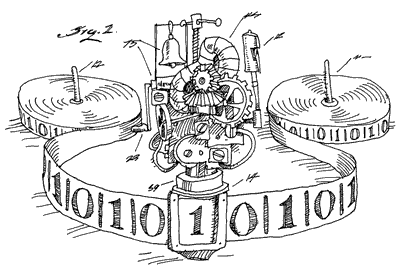
\includegraphics[scale=1]{turing/tmAufbau}
\end{frame}

% Kann ich erst Werbung für machen, nachdem ich ihn selbst gesehen habe, sonst wird's unglaubwürdig... :P
% Dann solltest du ihn unbedingt mal anschauen!
\thasse{
	\begin{frame}{Alan Turing}
		\centering
		\vspace{-25pt}
		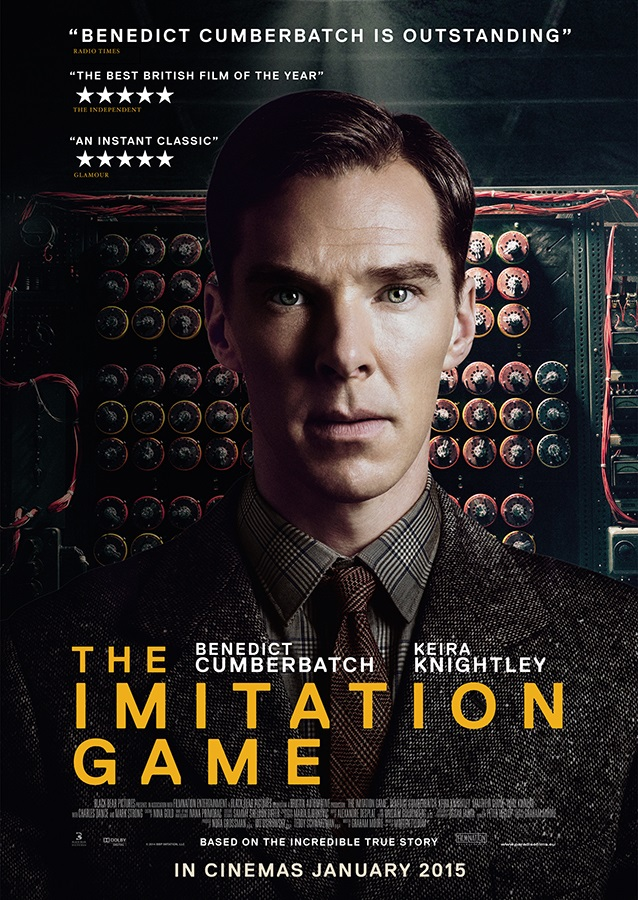
\includegraphics[scale=0.35]{turing/imitationGame}
	\end{frame}
}
} % end mycomment

%Das hier am Besten hinmalen mit Band und Schreiblesekopf und an der Tafel machen:
\begin{frame}{Eine einfache Turingmaschine}
	\begin{center}
		\begin{tikzpicture}[->,>=stealth,shorten >=1pt,auto,node distance=2.8cm,
		semithick,initial text={}]
		\tikzstyle{every state}=[]
		
		\node[initial,state] (A)                    {$a$};
		\node[state]         (M) [right of=A] 	    {$m$};
		
		\path 
		(A) edge [loop above] node {$\word 1\io\word 0R$} (A)
		edge [loop below]  node {$\word 0\io\word 1R$} (A)
		edge 					  node {$\word{2}\io\word{X}R$} (M)
		(M) edge [loop right] node {$\stackedtight{\word 0\io\word XR \\ \word 1\io\word XR \\ \word 2\io\word XR}$} (M)
		;
		\end{tikzpicture}
	\end{center} \pause
	Diese TM vertauscht $\word 1$en und $\word 0$en und ist beleidigt, wenn sie eine $\word 2$ liest. \\ \pause
	\begin{tabular}{rl@{\ \?>\ }rl}
		Zustand vorher: & a &  nachher: & \hphantom{\word{100010}}a \\
		Band vorher: &\word{011101} &  nachher:&  \word{100010}$\9$\\
		\hline
		Zustand vorher: & a &  nachher: & \hphantom{\word{100010}}m \\
		Band vorher: &\word{011102} &  nachher:&  \word{10001X}$\9$\\
		\hline
		Zustand vorher: & a &  nachher: & \hphantom{\word{100010}}m \\
		Band vorher: &\word{012101} &  nachher:&  \word{10XXXX}$\9$\\
	\end{tabular}

\end{frame}



\begin{frame}{Turingmaschinen}
	Eine Turingmaschine besteht aus...
	\begin{itemize}[<+->]
		\item einem unendlichen Band mit einzelnen Zellen, in denen jeweils genau ein Symbol aus dem Bandalphabet steht
		\item einem Schreib-/Lesekopf, der auf genau einer Bandzelle steht
		\item einer Steuerungseinheit (ähnlich zu einem Moore-Automat, mit der Ausgabe in den Übergängen), die sich in genau einem Zustand befindet
	\end{itemize}
\end{frame}

\begin{frame}{Funktionsweise der TM}
	In jedem Ausführungsschritt:
	\begin{itemize}[<+->]
		\item TM liest das Symbol, auf dem der Kopf steht
		\item Steuerung entscheidet über die Ausgabe, den Folgezustand und die Bewegung
		\item Ausgabe wird an der aktuellen Position auf das Band geschrieben
		\item Steuerung wechselt in den Folgezustand
		\item Kopf bewegt sich einen Schritt nach links (L) oder rechts (R) oder bleibt stehen (0)
	\end{itemize}
	\pause
	Die TM \textbf{hält}, wenn für einen Zustand und das gelesene Symbol keine Übergänge in der Steuerung definiert sind. \textbf{Eine TM muss nicht halten!} \\
	\impl Es können „Pfeile fehlen“!
\end{frame}

\begin{frame}{Eine einfache Turingmaschine v2}
	\begin{center}
		\begin{tikzpicture}[->,>=stealth,shorten >=1pt,auto,node distance=2.8cm,
		semithick,initial text={}]
		\tikzstyle{every state}=[]
		
		\node[initial,state] (A)                    {$a$};
		
		\path 
		(A) edge [loop above] node {$\word 1\io\word 0R$} (A)
		edge [loop below]  node {$\word 0\io\word 1R$} (A)
		;
		\end{tikzpicture}
	\end{center} \pause
	Pfeil für Eingabe \word 2 fehlt jetzt! \pause \impl TM hört dann einfach auf! \\ \pause
	\begin{tabular}{rl@{\ \?>\ }rl}
		Zustand vorher: & a &  nachher: & \hphantom{\word{100010}}a \\
		Band vorher: &\word{011101} &  nachher:&  \word{100010}$\9$\\
		\hline
		Zustand vorher: & a &  nachher: & \hphantom{\word{10001}}a \\
		Band vorher: &\word{011102} &  nachher:&  \word{100012}\\
		\hline
		Zustand vorher: & a &  nachher: & \hphantom{\word{10}}a \\
		Band vorher: &\word{012101} &  nachher:&  \word{102101}\\
	\end{tabular}
	
\end{frame}

\begin{frame}{Eine einfache Turingmaschine, Rage-Mode!}
	\begin{center}
		\begin{tikzpicture}[->,>=stealth,shorten >=1pt,auto,node distance=2.8cm,
		semithick,initial text={}]
		\tikzstyle{every state}=[]
		
		\node[initial,state] (A)                    {$a$};
		\node[state]         (M) [right of=A] 	    {$m_1$};
		\node[state]         (M2) [right of=M] 	    {$m_2$};
		
		\path 
		(A) edge [loop above] node {$\stackedtight{\word 1\io\word 0R \\ \word 0\io\word 1R}$} (A)
		edge 					  node {$\word{2}\io\word{2}R$} (M)
		(M) edge [loop above] node {$\stackedtight{\word 0\io\word 0R \\ \word 1\io\word 1R \\ \word 2\io\word 2R}$} (M)
		edge 					  node {$\9\io\9L$} (M2)
		(M2) edge [loop right] node {$\stackedtight{\word 0\io\9L \\ \word 1\io\9L \\ \word 2\io\9L}$} (M2)
		;
		\end{tikzpicture}
	\end{center} \pause
	\impl Löscht das komplette Eingabewort, wenn sie ne \word 2 in die Finger kriegt! \smiley \\ \pause
	\begin{tabular}{rl@{\ \?>\ }rl}
		Zustand vorher: & a &  nachher: & \hphantom{\word{100010}}a \\
		Band vorher: &\word{011101} &  nachher:&  \word{100010}$\9$\\
		\hline
		Zustand vorher: & a &  nachher: & $m_2$\\
		Band vorher: &\word{011102} &  nachher:&  $\9\9\9\9\9\9$\\
		\hline
		Zustand vorher: & a &  nachher: & $m_2$ \\
		Band vorher: &\word{012101} &  nachher:& $\9\9\9\9\9\9$\\
	\end{tabular}
\end{frame}

\begin{frame}{Ein-/Ausgabe}
	\begin{block}{Eingabe}
		Am Anfang steht das Eingabewort umgeben von Blanksymbolen auf dem Band, der Kopf steht auf dem ersten Zeichen des Eingabeworts.
	\end{block}
	\pause
	
	\begin{block}{Ausgabe}
		Zwei Möglichkeiten:
		\begin{itemize}[<+->]
			\item Berechnung von Funktionen: Ausgabewort steht am Ende auf dem Band \\
			\impl „normale“ TMen
			\item Erkennen von Sprachen: Halten in akzeptierendem Zustand (Doppelkringel)\\
			\impl Turingmaschinen-\textbf{Akzeptor} \\
				  Wir bezeichnen dann wieder mit $L(T)$ die akzeptierte Sprache \\
				  (Was aufm Band steht, ist dann bloß Nebenrechnung.)
		\end{itemize}
	\end{block}
\end{frame}

\begin{frame}{Konfigurationen}
	Den „Gesamtzustand“ einer Turingmaschine (also akt. Zustand, Bandinhalt und Schreibkopf-Position) nennen wir \textbf{Konfiguration}. \\ \pause
	\medskip
	In GBI schreiben wir dafür das aktuelle Wort auf dem Band und über das Zeichen, auf dem der Kopf grade steht, den Zustand. \\
	Beispiel: \\
	\bigskip
	\mbox{}\hphantom{\word{100}$\9$.\!}z \\
	\mbox{\word{100}$\9$\word{101}}
	
	\pause \bigskip
	(Formalkram dazu: \impl VL!)
\end{frame}

\mycomment{ %TODO Fix. Oder gleich an der Tafel machen erkläutern, wie das mit Konfigurationen geht. IMHO besser.
	\begin{frame}{Beispiel}
		\vspace{-30pt}
		\begin{center}
			
			\begin{tikzpicture}[shorten >=1pt,initial text=,node distance=2cm,auto,->,>=stealth,baseline=(B.base)]
			% \node[state,initial]  (S)                       {$S$};
			\node[state,initial]  (A)          {$A$};
			% \node (nix) [right of=A] {};
			\node[state]          (B) [above right of=A] {$B$};
			\node[state]          (C) [right of=B] {$C$};
			\node[state]          (E) [below right of=A] {$E$};
			\node[state]          (D) [right of=E] {$D$};
			\path[->]
			% (S) edge              node  {$\9\io\9R$} (A)
			(A) edge              node  {$\word 1\io\word XR$} (B)
			(B) edge [loop above] node  {$\word 1\io\word 1R$} ()
			edge              node  {$\9\io\9R$} (C)
			(C) edge [loop above] node  {$\word 1\io\word 1R$} ()
			edge              node  {$\9\io\word 1L$} (D)
			(D) edge [loop below] node  {$\word 1\io\word 1L$} ()
			edge              node  {$\9\io\9L$} (E)
			(E) edge [loop below] node  {$\word 1\io\word 1L$} ()
			edge              node  {$\word X\io\word 1R$} (A)
			% (B) edge              node        {$\9\io\9R$} (B)
			% edge [loop right] node        {$\#1\io\#1R$} ()
			% (B) edge [loop right] node {$\9\io\#1L$} ()
			% edge  node [pos=0.3]       {$\#1\io\#1L$} (A)
			;
			\end{tikzpicture}
			\bigskip
			
			\begin{tabular}{c|c|c|c|c|c}
				%	& A & B & C & D & E \\ \hline
				%	$\square $ & & C,$\square$,R & D, $\word 1$, L & E,$\square$, L & \\ \hline
				%	$\word 1$ & B,$X$, R & B,$\word 1$, R & C,$1$, R & D,$\word 1$, L & E,$\word 1$, L \\ \hline
				%	$X$ & & & & & A,$\word 1$,R \\
			\end{tabular}
		\end{center}
	\end{frame}
	
	% DIESES BEISPIEL IST FEHLERHAFT!
	\begin{frame}[t]{Beispiel}
		\only<1|handout:1>{Eingabe: $11$}
		\bigskip
		\begin{itemize}
			\only<1-3|handout:1>{\item[1] \begin{Messtabelle}{ccccccc} & A & & & & & \\ & $\downarrow$ &&&&& \\ 
					$\square$ & 1 & 1 & $\square$ & $\square$ & $\square$ & $\square$ \end{Messtabelle} }
			\only<2-4|handout:1>{\item[2] \begin{Messtabelle}{ccccccc} &  & B & & & & \\ & &$\downarrow$ &&&& \\ 
					$\square$ & X & 1 & $\square$ & $\square$ & $\square$ & $\square$ \end{Messtabelle} }
			\only<3-5|handout:1>{\item[3] \begin{Messtabelle}{ccccccc} &  & & & C& &  \\ &  &&& $\downarrow$ & &\\ 
					$\square$ & X & 1 & $\square$ & $\square$ & $\square$ & $\square$ \end{Messtabelle} }
			\only<4-6|handout:2>{\item[4] \begin{Messtabelle}{ccccccc} &  & & D & & &  \\ &  && $\downarrow$ &&& \\ 
					$\square$ & X & 1 & $\square$ & 1 & $\square$  & $\square$ \end{Messtabelle} }
			\only<5-7|handout:2>{\item[5]  \begin{Messtabelle}{ccccccc} &  & E &  & & &  \\ &  & $\downarrow$ &&&& \\ 
					$\square$ & X & 1 & $\square$ & 1 & $\square$  & $\square$ \end{Messtabelle} }
			\only<6-8|handout:2>{ \item[6] \begin{Messtabelle}{ccccccc} &  &   A && & &  \\ &  &  $\downarrow$ &&&& \\ 
					$\square$ & 1 & 1 & $\square$ & 1 & $\square$  & $\square$ \end{Messtabelle} }
			\only<7-9|handout:3>{\item[7] \begin{Messtabelle}{ccccccc} &  &    & B & & &  \\ &  &&  $\downarrow$ &&& \\ 
					$\square$ & 1 & X & $\square$ & 1 & $\square$  & $\square$ \end{Messtabelle} }
			\only<8-10|handout:3>{\item[8] \begin{Messtabelle}{ccccccc} &  &    &  & & C &  \\ &  && && $\downarrow$ & \\ 
					$\square$ & 1 & X & $\square$ & 1 & $\square$  & $\square$ \end{Messtabelle} }
			\only<9-11|handout:3>{\item[9] \begin{Messtabelle}{ccccccc} &  &    &  &  D& &  \\ &  && & $\downarrow$ && \\ 
					$\square$ & 1 & X & $\square$ & 1 & 1  & $\square$ \end{Messtabelle} }
			\only<10-12|handout:4>{\item[10] \begin{Messtabelle}{ccccccc} &  &   E &  &  & &  \\ &   & $\downarrow$ && &&\\ 
					$\square$ & 1 & X & $\square$ & 1 & 1  & $\square$ \end{Messtabelle} }
			\only<11-12|handout:4>{\item[11] \begin{Messtabelle}{ccccccc} &  &    & A &  & &  \\ &   && $\downarrow$ && &\\ 
					$\square$ & 1 & 1 & $\square$ & 1 & 1  & $\square$ \end{Messtabelle} }
		\end{itemize}
		\only<12|handout:4>{ Also allgemein : Eingabe von $1^k$ wird zu $\square \, 1^k \, \square \, 1^k \, \square $} 
	\end{frame}
}


\begin{frame}{Turingmaschine}
	\begin{Definition}
		Eine Turingmaschine $T$ ist definiert als $$ T = (Z, z_0 , X, f,g, m)$$
		\begin{itemize}[<+->]
			\item $Z \quad$ Zustandsmenge 
			\item $z_0\in Z \quad$ Startzustand
			\item $X \quad$ Bandalphabet mit $\square \in X$
			\item $f:Z\times X \dashrightarrow Z \quad$ Übergangsfunktion
			\item $g:Z\times X\dashrightarrow X \quad$ Ausgabefunktion  \quad (\textbf{genau ein Zeichen} als Ausgabe!)
			\item $m:Z\times X \dashrightarrow \{\text{L},\text{0},\text{R}\} \quad$ Bewegungsfunktion
		\end{itemize}
		\pause
		Alle Funktionen können auch nur partiell definiert ($\dashrightarrow$) sein. \\
		(Heißt: Sie sind nicht linkstotal $=$ Es fehlen Pfeile.)
	\end{Definition}
\end{frame}

\begin{frame}{Beispiel: Formale Definition}
	\begin{center}
		\begin{tikzpicture}[->,>=stealth,shorten >=1pt,auto,node distance=2.8cm,
		semithick,initial text={}]
		\tikzstyle{every state}=[]
		
		\node[initial,state] (A)                    {$a$};
		\node[state]         (M) [right of=A] 	    {$m_1$};
		\node[state]         (M2) [right of=M] 	    {$m_2$};
		
		\path 
		(A) edge [loop above] node {$\stackedtight{\word 1\io\word 0R \\ \word 0\io\word 1R}$} (A)
		edge 					  node {$\word{2}\io\word{2}R$} (M)
		(M) edge [loop above] node {$\stackedtight{\word 0\io\word 0R \\ \word 1\io\word 1R \\ \word 2\io\word 2R}$} (M)
		edge 					  node {$\9\io\9L$} (M2)
		(M2) edge [loop right] node {$\stackedtight{\word 0\io\9L \\ \word 1\io\9L \\ \word 2\io\9L}$} (M2)
		;
		\end{tikzpicture}
	\end{center}
	\begin{align*}
		\text{Bandalphabet } X &= \set{\word 0, \word 1, \word 2, \9} \\
		f(a,\word 1) &= a	\\
		f(a, \9) &\text{ ist nicht definiert.} \\ 
		g(a, \word 1) &= \word 0 \\
		g(a, \9) &\text{ ist nicht definiert.} \\ 
		m(m_1, \9) &= L \\
		m(m_2, \9) & \text{ ist nicht definiert.}
	\end{align*}
\end{frame}

\begin{frame}{Aufgabe}
	Was macht die folgende Turingmaschine für Eingaben aus $\{\word 0, \word 1\}^*$?
	
	%\smallskip
	%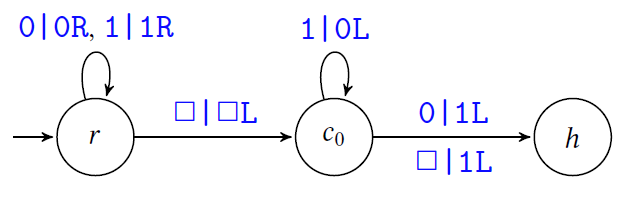
\includegraphics[scale=0.65]{turing/addBin1}
	\begin{center}
		\begin{tikzpicture}[->,>=stealth,shorten >=1pt,auto,node distance=2.8cm,
		semithick,initial text={}]
		\tikzstyle{every state}=[]
		
		\node[initial,state] (R)                    {$r$};
		\node[state]         (C) [right of=R] 	    {$c_0$};
		\node[state]         (H) [right of=C] 	    {$h$};
		
		\path 
		(R) edge [loop above] node {$\word 0\io\word 0R, \word 1\io\word1R$} (R)
		edge 					  node {$\9\io\9L$} (C)
		(C) edge [loop above] node {$\word 1\io\word 0L$} (C)
		edge 					  node {$\stackedtight{\word 0\io\word 1L, \\ \9\io\word 1L }$} (H)
		;
		\end{tikzpicture}
	\end{center}
	
	\smallskip
	\visible<2|handout:2>{
		Inkrementieren der dargestellten Zahl um $1$.
	}
\end{frame}

\begin{frame}{Aufgabe}
	Entwerft eine Turingmaschine, die für eine Eingabe $w \in \{\word 0, \word 1\}^*$ $$\fRepr_2(\fNum_2(w) - 1)$$ berechnet. Ihr dürft davon ausgehen, dass $\fNum_2(w) > 0$ gilt.\\
	\visible<2-|handout:2->{
		\begin{center}
			\begin{tikzpicture}[->,>=stealth,shorten >=1pt,auto,node distance=2.8cm,
			semithick,initial text={}]
			\tikzstyle{every state}=[]
			
			\node[initial,state] (R)                    {$r$};
			\node[state]         (C) [right of=R] 	    {$c_0$};
			\node[state]         (H) [right of=C] 	    {$h$};
			
			\visible<4-|handout:3->{
				\node[state]         (Z) [below=1cm of H] 	    {$z$};
			}
			\visible<6-|handout:4->{
				\node[state]         (L) [below=1cm of C] 	    {$\ell$};
			}
			
			\path 
			(R) edge [loop above] node {$\word 0\io\word 0R, \word 1\io\word1R$} (R)
			edge 					  node {$\9\io\9L$} (C)
			(C) edge [loop above] node {$\word 0\io\word 1L$} (C)
			edge 					  node {$\word 1\io\word 0L$} (H);
			
			\visible<4-|handout:3->{
				\path
				(H) edge [loop above] node {$\word 0\io\word 0L, \word 1\io\word1L$} (H)
				edge [left]				  node {$\9\io\9R$} (Z)
				(Z)  edge [loop right] node {$\word 0\io\9R$} (Z);
			}
			
			\visible<6-|handout:4->{
				\path
				(Z)  edge 				 node[below] {$\9\io\word 0L$} (L);
			}
			\end{tikzpicture}
		\end{center}
	}
	\visible<3-|handout:3->{\§{\textbf{Achtung}:} Was passiert mit führenden Nullen?} \\ 
	\visible<5-|handout:4->{\. Was, wenn es nur eine \word 0 gibt?} \\	
\end{frame}

\begin{frame}{Aufgabe}
	Wie würde man eine (einfache, nicht effiziente) TM zum Addieren von zwei Zahlen in Binärdarstellung aufbauen? \\ \pause
	\smallskip
	\impl Inkrementiere erste Zahl, dekrementiere zweite Zahl. Wiederhole, bis zweite Zahl $= 0$.
\end{frame}

\def\bword#1{\texttt{#1}}
\begin{frame}[t]{TM-Akzeptoren}
	\only<all:1>{
		Erinnerung: Inkrementieren um eins 
		\begin{center}
			\begin{tikzpicture}[->,>=stealth,shorten >=1pt,auto,node distance=2.8cm,
				semithick,initial text={}]
				\tikzstyle{every state}=[]
				
				\node[initial,state] (R)                    {$r$};
				\node[state]         (C) [right of=R] 	    {$c_0$};
				\node[state]         (H) [right of=C] 	    {$h$};
				
				\node[state,accepting,white]         (A) [below of=H] 	    {\phantom{$a_1$}};
				\node[state,white]         (B) [below of=C] 	    {\phantom{$a_2$}};
				
				\path 
				(R) edge [loop above] node {$\word 0\io\word 0R, \word 1\io\word 1R$} (R)
				edge 					  node {$\9\io\9L$} (C)
				(C) edge [loop above] node {$\word 1\io\word 0L$} (C)
				edge 					  node {$\stackedtight{\word 0\io\word 1L \\ \9\io\word 1L}$} (H)
				
				(H) edge [loop above,white] node {\phantom{$\word 0\io\word 0L, \word 1\io\word 1L$}} (H)
				(A)  edge [white]				 node[below] {\phantom{$\word 0\io\word 0L$}} (B)
				;
			\end{tikzpicture}
		\end{center}
	\mbox{}\vphantom{Welche Sprache....} \\
	}
	\only<all:2->{
		\?> TM-Akzeptor: 
		\begin{center}
			\begin{tikzpicture}[->,>=stealth,shorten >=1pt,auto,node distance=2.8cm,
				semithick,initial text={},every initial by arrow/.style={gray}]
				\tikzstyle{every state}=[]
				
				\node[initial,state,gray] (R)                    {$r$};
				\node[state,gray]         (C) [right of=R] 	    {$c_0$};
				\node[state]         (H) [right of=C] 	    {$h$};
				
				\node[state,accepting]         (A) [below of=H] 	    {$a_1$};
				\node[state]         (B) [below of=C] 	    {$a_2$};
				
				\path 
				(R) edge [loop above,gray] node {$\bword 0\io\bword 0R, \bword 1\io\bword 1R$} (R)
				edge [gray] 					  node {$\9\io\9L$} (C)
				(C) edge [loop above,gray] node {$\bword 1\io\bword 0L$} (C)
				edge [gray] 					  node {$\stackedtight{\bword 0\io\bword 1L \\ \9\io\bword 1L}$} (H)
				
				(H) edge [loop above] node {$\word 0\io\word 0L, \word 1\io\word 1L$} (H)
				edge [left]				  node {$\9\io\9R$} (A)
				(A)  edge [loop above left] node[left] {$\word 1\io\word 1R$} (A)
				(A)  edge 				 node[below] {$\word 0\io\word 0R$} (B)
				;
			\end{tikzpicture}
		\end{center}
		Welche Sprache akzeptiert diese TM? \\
	}
	\medskip
	\visible<3-|handout:2->{$\impl L(T) = \set{w \in \set{\word 0,\word 1}^* \Mid \fRepr_2(\fNum_2(w) + 1) \in \set{\word 1}^*}$}
\end{frame}

\begin{frame}{Turing-Maschinen vs. Supercomputer}
	Eine TM kann \textbf{genauso viel} berechnen wie euer Handy oder ein Supercomputer von Intel. {\small (Bloß halt etwas langsamer und umständlicher!)} \\
	\medskip
	Es gibt kein „mächtigeres“ Maschinenmodell als Turingmaschinen. \\
	\only<beamer:0>{
		\medskip 
		\begin{center}
			\impl Was eine Turingmaschine nicht berechnen \\ kann, kann keiner berechnen. \smiley \\ \#Prädikatenlogik-Blatt 2017/18
		\end{center}
	}
\end{frame}

\mycomment{ % Formalkram ist bähhh...
	% Ja, aber eigentlich wichtig. Aber dieses Jahr keine Zeit.
	\begin{frame}{Konfiguration}
		\begin{Definition}
			Als \textbf{Konfiguration} $ c =(z,b,p)$ bezeichnen wir den Zustand einer Turing-Maschine zu einem Zeitpunkt. Dabei ist 
			\begin{itemize}
				\item $z\in Z$ der Zustand
				\item $b: \Z\to X$ die Bandbeschriftung
				\item $p\in \Z$ die Position des Zeigers.
			\end{itemize}
		\end{Definition}
	\end{frame}
	
	\begin{frame}{Berechnungsschritte}
		\begin{Definition}
			In einem Berechnungsschritt geht eine TM aus einer Konfiguration $c$ 
			in die Konfiguration $$\Delta_1(c) := c' = (z',b',p')$$ über, wobei gilt:
			\begin{itemize}[<+->]
				\item $z' = f(z,b(p))$
				\item $\forall i\in \Z: b'(i) =
				\begin{cases}
				b(i) & \text{ falls } i\not=p \\
				g(z,b(p)) & \text{ falls } i=p
				\end{cases}$
				\item $p' = p + m(z,b(p))$
			\end{itemize}
			\bigskip
			
			\pause
			Wenn $\Delta_1(c)$ nicht definiert ist, bezeichnet man $c$ als \textbf{Endkonfiguration} und die TM \textbf{hält}.
		\end{Definition}
	\end{frame}
	
	\begin{frame}{Berechnungen}
		\begin{Definition}
			Eine Berechnung ist eine Folge von Konfigurationen $(c_0, c_1, ..., c_t)$ bei der gilt $$c_{i+1} = \Delta_1(c_i)$$ \pause
			Es gibt endliche, haltende (endet in einer Endkonfiguration) und unendliche Berechnungen.
			\bigskip
			
			\pause
			Induktiv definiert man $\Delta_t(c) , t\in\N_0$ als die Konfiguration, welche nach $t$ Berechnungsschritten erreicht werden kann und $\Delta_*(c)$ als Endkonfiguration, die von $c$ aus erreicht wird (falls die Berechnung endet).
		\end{Definition}
	\end{frame}
}








\begin{frame}{Entscheidbarkeit}
	\begin{Definition}
		Eine Sprache $L$ ist eine   
		\begin{itemize}[<+->]
			\item \textbf{aufzählbare Sprache}, wenn es eine Turingmaschine gibt, die $L$ akzeptiert.
			\item \textbf{entscheidbare Sprache}, wenn es eine Turingmaschine gibt, die $L$ akzeptiert und \emph{für jede Eingabe} hält.
		\end{itemize}
	\end{Definition} \pause
	
	Bei aufzählbaren Sprachen ist nicht definiert, wie sich die TM für Wörter $ w \notin L$ verhält. Sie kann diese ablehnen oder nicht halten. Ob eine TM für eine Eingabe nicht hält, können wir \enquote{von außen} nicht einfach feststellen.
\end{frame}


\begin{frame}{Aufgabe}
	Entwerft eine Turingmaschine, die die Sprache $ \{\word 0^k\word 1^k \mid k\in \N_0 \} $ akzeptiert.
	% TODO Lösung
\end{frame}

\begin{frame}{Aufgabe}
	Entwerft eine TM, die alle gültigen Klammerausdrücke entscheidet.\\
	\medskip
	Gültige Klammerausdrücke werden dabei von der folgenden Grammatik produziert: $ G = (\{S\},\{\word (, \word )\}, S, P )$ mit den Produktionen $\set{ S \to \eps \mid \word (S\word )S}$.
	% TODO Lösung
\end{frame}


% Hier CS50 Binary Search (Telefonbuchszene) zeigen! (Spulen!!!)
% https://www.youtube.com/watch?v=o4SGkB_8fFs&list=PLhQjrBD2T382VRUw5ZpSxQSFrxMOdFObl

% Live kam das ganze bisher immer sehr gut an, also wer ein Telefonbuch hat...
% Video geht aber auch, es braucht also nicht zwingend ein Telefonbuch...
% Aber wer eines hat (die Post hat welche!), Live wäre das ganze natürlich schon besser...

% QUESTION (DJ): Wieso hier? Mastertheorem ist doch erst später?
% ANSWER   (TH): Geht auch gar nicht mit dem vereinfachten MT aus dem Tut.
%                Es geht hier eher darum, zur Motivation ein Gefühl für "es gibt langsame und schnelle Algorithmen" zu entwickeln 
%                und außerdem binäre Suche zu verstehen, und wie logarithmische Laufzeiten entstehen und warum sie toll sind.

%\section{Quantitative Aspekte}

% TODO: Mehr und bessere Beispiele, generelle Überarbeitung (VL-Folien)

\subsection{Motivation}
\begin{frame}{Laufzeiten}
	Wir interessieren uns für Laufzeiten von Algorithmen.
	\pause
	\begin{itemize}
		\item Aber wie sollen wir die messen?
		\item Problem: Rechenzeit auf einem Supercomputing-Cluster nicht mit Rechenzeit auf einem IoT-Chip in der Waschmaschine vergleichbar
		\implitem Zählen der \enquote{ausgeführten Operationen} in Abhängigkeit von der Problemgröße $n$
		\item Noch ein Problem: Genaue Anzahlen sind seeehr schwierig zu bestimmen...
		\item[] ... und in vielen Fällen auch irrelevant
		\implitem konstante Faktoren ignorieren!
	\end{itemize}
\end{frame}

%% -----------------------------------------------------------------------------

\subsection{Definitionen}
\begin{frame}{Asymptotisches Wachstum}
	\begin{Definition}
		Zwei Funktionen $f,g: \N_0 \to \R_0^+$ wachsen asymptotisch gleich schnell, wenn es zwei Konstanten $c, c' \in \R^+$ gibt, so dass gilt $$\exists n_0 \in \N_0: \ \forall n \geq n_0: \ c \* f(n) \leq g(n) \leq c' \* f(n) $$
		Man schreibt dafür 
		\begin{align*}
			f &\asymp g \\
			\textbf{oder} \quad f(n) &\asymp g(n) 
			% Hashtag: „n^2“ ist ein Term und keine Funktion etc... Man müsse doch [n \mapsto n^2] schreiben... VL erlaubt ersteres aber auch.
		\end{align*}
	\end{Definition} \pause
	Diese Relation ist eine Äquivalenzrelation!
\end{frame}

\begin{frame}{Landau-Notation I}
	\begin{Definition}
		$\Theta(f)$ ist die Menge aller Funktionen $g$, die asymptotisch genauso schnell wachsen wie $f$, also $$\Theta(f) := \{ g \mid f \asymp g \}$$
	\end{Definition}
	
	\medskip
	\only<1|handout:1>{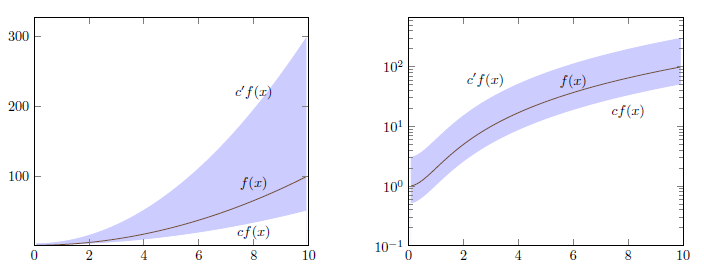
\includegraphics[scale=0.6]{laufzeit/theta1}}
	\only<2|handout:2>{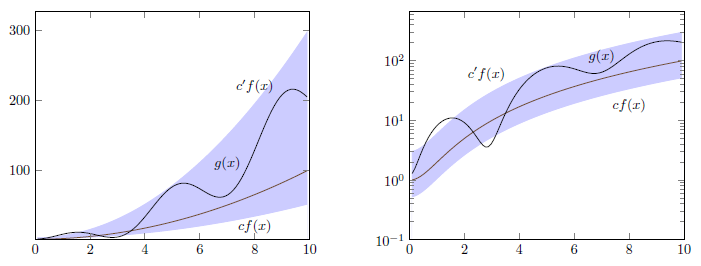
\includegraphics[scale=0.6]{laufzeit/theta2}}
\end{frame}

\begin{frame}{Beispiel 1}
	Seien \quad $f(n) := 2 \cdot n^2 + n, \qquad g(n) := n^2.$ \\
	\textbf{Behauptung:} \quad $ f \in \Th{g} $. \\ 
	\medskip \pause
	\textbf{Beweis:} \quad Wir suchen $n_0, c, c'$ mit $\forall n \geq n_0: \ c \* g(n) \leq f(n) \leq c' \* g(n) $.
	\smallskip \pause
	
	Sei $n \geq 1$, so gilt: \pause 
	\begin{align*}
	f(n) &= 2 \cdot n^2 + n \leq 2 \cdot n^2 + n^2 = 3 \cdot n^2 = 3 \cdot g(n)\quad \text{ und} \\ 
	\visible<5->{f(n) &= 2 \cdot n^2 + n \geq 2 \cdot n^2 = 2 \cdot g(n).}
	\end{align*}
	\pause % I hate you, LaTeX. -.-
	Mit $c := 2$, \, $c' := 3$,\, $n_0 := 1$ ist die Bedingung erfüllt. \qed \pause
	
	\begin{block}{Quiz}
		\TrueQuestion{$n^{100} + 10^9 n^{99} \in \Th{n^{100}}$}
		\FalseQuestion{$2^n \in \Th{n^2}$}
	\end{block}
\end{frame}

\begin{frame}{Beispiel 2}
	\textbf{Behauptung:} \quad $  \sin(n) + 2 \elem \Th{1} $ \\ \medskip \pause
	\textbf{Beweis:} \quad Wähle $c := 1, \, c' := 3, \, n_0 := 0$.  \quad Dann gilt $\forall n \geq n_0$: \\
	\begin{align*}
	c \* 1 = 1 &\leq \sin(n) + 2 \leq 3 = c' \* 1 \\
	\text{\Gdw} \qquad  -1 &\leq \sin(n) \leq 1. \qed
	\end{align*}
	\pause
	\Impl Der Sinus ist also „ungefähr“ konstant\only<handout>{ (wenn man seine Brille absetzt \smiley)}.
\end{frame}

\begin{frame}{Asymptotisches Wachstum}
	\begin{Definition}
		Für zwei Funktionen $f,g: \N_0 \to \R_0^+$ definiert man:
		$$g \preceq f \Gdw \exists c \in \R^+ \ \exists n_0 \in \N_0 \ \forall n \geq n_0: \ g(n) \leq c \* f(n)$$
		$$g \succeq f \Gdw \exists c \in \R^+ \ \exists n_0 \in \N_0 \ \forall n \geq n_0: \ g(n) \geq c \* f(n)$$
		(Schreibe analog auch $g(n) \preceq f(n)$ etc.)
	\end{Definition} \pause
	Diese Relationen sind \textbf{keine} Äquivalenzrelationen!
\end{frame}

\begin{frame}[t]{} % erased title due to \includepdf madness... I guess it's not that important anyway. Tags: fake title faketitle include pdf frametitle
	\fakeframetitle{Landau-Notation II}
	\begin{Definition}
		$\Oh{f}$ ist die Menge aller Funktionen $g$, die asymptotisch höchstens so schnell wachsen wie $f$, also $$\Oh{f} := \{ g \mid g \preceq f \}$$
		$\Om{f}$ ist die Menge aller Funktionen $g$, die asymptotisch mindestens so schnell wachsen wie $f$, also $$\Om{f} := \{ g \mid g \succeq f \}$$
	\end{Definition} \pause
	\impl $O$ ist eine Abschätzung nach oben. $\Omega$ ist eine Abschätzung nach unten.
\end{frame}


%\setbeamercolor{background canvas}{bg=}
%
\includepdf[pages=15]{U11.pdf}

\mycomment{ % let's not even teach them that this exists. Mentioning it in the lecture is enough
\begin{frame}{Eine katastrophale Schreibweise}
	Manchmal (häufig) sieht man auch das, \textbf{NICHT VERWENDEN}:
	$$f = \Theta(g) \qquad h = \Oh{n^3} \qquad k = \Omega(f + g)$$
	\pause
	Dabei das „$=$“ immer als „$\in$“ lesen!
\end{frame}
}

\begin{frame}[t]{} % fake title
	\fakeframetitle{Aufgabe: Inklusionen}
	Ordnet folgende Funktionen nach asymptotischem Wachstum an:
	\begin{itemize}
		\item Identität $f(x) = x$
		\item Konstante Funktion $f(x) = c$
		\item Wurzel
		\item Exponentialfunktion
		\item Logarithmus
	\end{itemize}
\end{frame}

%% Übung: Asymptotische Visualisierungen verschiedener Funktionen
\setbeamercolor{background canvas}{bg=}

\includepdf[pages={5-10}]{U11.pdf}

%\begin{frame}
%	\frametitle{Grenzwertabschätzung}
%	Wir können das auch anders schreiben:
%	\begin{align*}
%	f \in O(g) \qquad &\iff & \qquad 0 \leq  \limsup \limits_{n \to \infty} \frac{f(n)}{g(n)} < \infty \\
%	f \in \Omega(g) \qquad &\iff & \qquad 0 < \liminf  \limits_{n \to \infty} \frac{f(n)}{g(n)} \leq \infty \\
%	f \in \Theta(g) \qquad & \iff & \qquad 0 <  \liminf  \limits_{n \to \infty} \frac{f(n)}{g(n)} \leq  \limsup \limits_{n \to \infty} \frac{f(n)}{g(n)} < \infty
%	\end{align*} \pause
%	Oftmals existiert sogar $\lim$ und wir können $\liminf$ und $\limsup$ vergessen!
%\end{frame}
%
%\begin{frame}{Satz von L'Hospital}
%	\begin{block}{Satz}
%		Gegeben sei $$ \limes{x\to x_0} \frac{f(x)}{g(x)} $$ mit $$ \limes{x\to x_0} f(x) = \limes{x\to x_0} g(x) = 0 \vee \limes{x\to x_0} f(x) = \limes{x\to x_0} g(x) = \infty $$ 
%		Dann gilt 
%		$$ \limes{x\to x_0} \frac{f(x)}{g(x)} = \limes{x\to x_0} \frac{f'(x)}{g'(x)}   $$ mit 
%		$$ f'(x_0) = \left. \frac{\partial f(x)}{\partial x} \right|_{x=x_0} $$ 
%	\end{block}
%\end{frame}
%
%\begin{frame}{Beispiele}
%	Gilt $$ \log n \in \O \left(\sqrt{n}\right) $$ \pause 
%	Betrachte
%	\begin{align*}
%		\limes{n\to\infty} \log n &= \infty \\
%		\limes{n\to\infty} \sqrt{n} &= \infty \\
%		\frac{\partial \log n}{\partial n} &= \frac{1}{n} \\
%		\frac{\partial \sqrt{n}}{\partial n} &= \frac{1}{2} \frac{1}{\sqrt{n}} \\
%		\limes{n\to\infty} \frac{\log n}{\sqrt{n}} &= \limes{n\to\infty} \frac{\frac{1}{n}}{\frac{1}{2} \frac{1}{\sqrt{n}}} \\
%		&= 2 \limes{n\to\infty} \frac{\sqrt{n}}{n}  = 2 \limes{n\to\infty} \frac{1}{\sqrt{n}} = 0 
%	\end{align*}
%\end{frame}

%\subsection{Beispiele}
%\begin{frame}{Polynome}
%	Betrachten wir zwei Polynome $f(n) = n^4 + n^3$ und $g(n) = n^2$: \\
%	Der Quotient $$\frac{f(n)}{g(n)} = \frac{n^4 + n^3}{n^2} = n^2 + n \to \infty$$ Also ist $\lim f/g > 0$ und damit $$g \in O(f) \qquad f \in \Omega(g)$$ aber $\lim f/g = \infty$ also $$f \not \in O(g) \qquad g \not \in \Omega(f)$$ und vor allem $$f \not \in \Theta(g)$$
%\end{frame}

\begin{frame}{Logarithmen}
	\only<handout:0>{Informatiker LIEBEN Logarithmen...\\}
	\begin{block}{Einige Rechenregeln}
		\begin{align*}
			a^{\log_a n} &= n\\
			\visible<2-|handout:1>{\log_b (n \cdot m) &= \log_b n + \log_b m\\ 
			\log_b n^a &= a \cdot \log_b n\\}
			\visible<3-|handout:1>{a^{\log_b n} &= n^{\log_b a}}
		\end{align*}
	\end{block}
\end{frame}

\begin{frame}{Logarithmen}
	\begin{block}{Lemma}
		$$a^{\log_b n} = n^{\log_b a}$$
	\end{block} \pause

	\begin{block}{Herleitung}
		\begin{align*}
			a^{\log_b n} &= \left( b ^{\log_b a} \right) ^{\log_b n}\\
						 &= b^{\log_b a \, \cdot \, \log_b n}\\
						 &= \left( b^{\log_b n} \right) ^{\log_b a}\\
						 &= n^{\log_b a}
		\end{align*}
	\end{block}
\end{frame}

\begin{frame}{Logarithmen: Die Basis ist egal}
	\begin{block}{Lemma}
		$$ \log_a n \in \Th{\log_b n} $$
	\end{block}
	
	\begin{block}{Herleitung}
		Es gilt $$n = a^{\log_a n}$$ \pause
		Daraus ergibt sich: $$ \log_b n = \log_b \left(a^{\log_a n}\right) = \log_a n \; \cdot \log_b a $$ \pause 
		Setze $c = c' = \log_b a$, dann ist $$c \* \log_a n \leq \log_b n \leq c' \* \log_a n.$$
	\end{block}
\end{frame}

\begin{frame}{Logarithmen: Übung}
	\begin{block}{Einige Rechenregeln}
		\begin{align*}
			a^{\log_a n} &= n\\
			\log_b (n \cdot m) &= \log_b n + \log_b m\\ 
			\log_b n^a &= a \cdot \log_b n\\
			a^{\log_b n} &= n^{\log_b a}
		\end{align*}
	\end{block}

	\begin{block}{Aufgabe}
		\begin{align*}
			\log_5(25 \cdot 125) &= \visible<2->{\log_5(25) + \log_5(125) = 2+3 = 5}\\
			16^{\log_4(5)} &= \visible<3->{5^{\log_4(16)} = 5^2 = 25}
		\end{align*}
	\end{block}
\end{frame}

\begin{frame}{Rechenregeln (I)}
	Einige Rechenregeln im $O$-Kalkül
	\begin{itemize}[<+->]
		\item Für $a > 0$ ist $a \cdot f \in \Th{f}$ 
		\item Für Konstanten $c, d \geq 0$ gilt: \\ 
			\quad $f(n) \in \Oh{g(n)} \Impl f(n) + c \in \Oh{g(n) + d}$ \\
			\quad $f(n) \in \Om{g(n)} \Impl f(n) + c \in \Om{g(n) + d}$ \\
		\item Für $0 < a < b$ ist $n^a \preceq n^b$
		\item Für $a,b > 1$ ist $n^a \preceq b^n$ \qquad {\small (Exponentialfktnen. wachsen stärker als Polynome)}
		\item Für Polynome $f,g$ gilt: \\
			\quad $\mathop{\text{grad}} f = \mathop{\text{grad}} g \iff f \asymp g $
		\item Für $a,b > 0$ gilt $\log_a(n) \in \Theta(\log_b n)$
		
	\end{itemize}
\end{frame}


\begin{frame}{Rechenregeln (II)}
	Weitere Rechenregeln im $O$-Kalkül:
	\begin{itemize}[<+->]
		\item $f \in O(g) \iff g \in \Omega(f)$
		\item $\Theta(f) = O(f) \cap \Omega(f)$ und $f \asymp g \iff f \preceq g \wedge f \succeq g$ 
		\item $O(f_1) + O(f_2) = O(f_1 + f_2)$
		\item Wenn $g \in O(f)$, dann ist auch $O(g) \subseteq O(f)$ und $O(f + g) = O(f)$
	\end{itemize}

	\begin{block}{Kurze Aufgabe}
		Zeigt mit den Rechenregeln: Wenn $g\preceq f$, $h \succeq f$ und $h\in\Oh{g}$, dann ist $f \asymp g \asymp h$.
	\end{block}
\end{frame}

% TODO Aufgaben !!!!

%\subsection{Laufzeiten Angeben}
%
%\begin{frame}[fragile]
%	\frametitle{Algorithmus}
%		\verb+int x = 1;+ \\
%		\verb/for (int i = 0; i < n; i++) {/ \\
%		\verb+	x = a * x;+ \\
%		\verb+}+ \\
%		\verb+return(x);+ \\[1em]
%		 \pause
%	Was tut der? \pause Welche Laufzeit hat er?
%\end{frame}
%
%\begin{frame}[fragile]
%	\frametitle{Laufzeiten}
%		\verb+int x = 1;+ \\ \pause $O(1)$ \\ \pause
%		\verb/for (int i = 0; i < n; i++) {/ \\  \pause $O(1), O(1)$ \\ \pause
%		\verb+	x = a * x;+ \\  \pause $O(1)$ \\ \pause
%		\verb+}+ \\  \pause $n$-mal \\ \pause
%		\verb+return(x);+ \\  \pause $O(1)$ \\ \pause
%		 \pause
%		$$O(1 + n + n + 1) = O(n)$$
%\end{frame}


\begin{frame}	
	\begin{block}{Was ihr nun wissen solltet}
		\begin{itemize}
			\item Rechtslineare Grammatiken und Reguläre Ausdrücke
			\item Aufbau + Funktion von Turingmaschinen
			\item Entscheidbarkeit und Aufzählbarkeit
		\end{itemize}
	\end{block}
	
	\begin{block}{Was nächstes Mal kommt}
		\begin{itemize}
			\item Vorschriften zum Rechnen: Algorithmen
			\item Lizenz zum Schludern: O-Kalkül
			\item Einfache Laufzeitabschätzungen
			%TODO nexttut
			%\item Grenzen endlicher Automaten -- Wer kann zählen?
			%\item Ein Regelwerk für einen Ausdruck -- Reguläre Ausdrücke
		\end{itemize}
	\end{block}
\end{frame}

\xkcdframevert{612}{Danke für eure Aufmerksamkeit! \smiley}{2.5}
%\lastframe{0.65}{15}{xkcd/file_transfer_612.png}{http://www.xkcd.com/612}
\slideThanks

\end{document}